\documentclass[twocolumn]{article}

\usepackage{tikz}
\usepackage{amsmath}
\usepackage{pgfplots}

\begin{document}

\title{AP Physics C: Impulse Lab}
\author{Raja Williams}
\date{February 2024}
\maketitle

\section{Objective}
The Impulse Lab objective is to utilize impulse to experimentally determine the mass
of a sensor cart.

\section{Procedure}
\begin{enumerate}

    \item Record the ID present on the cart, for locating the cart later.

    \item Measure and record the mass of the cart.
    
    \item Set up half-Atwood machine with a 20 gram mass. Setup is visible in
        Figure \ref{fig:atwood}.

        \begin{figure}[h]
            \centering
            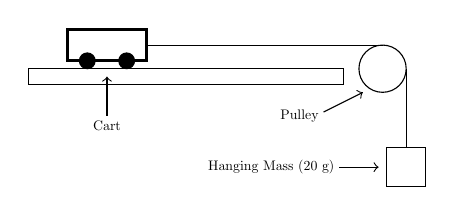
\begin{tikzpicture}[scale=0.5,transform shape]
                \draw[very thick] (0,0.2) rectangle (-2,1);
                \draw[fill=black] (-1.5,0.2) circle [radius=0.2];
                \draw[fill=black] (-0.5,0.2) circle [radius=0.2];
                \draw (6,0) circle [radius=0.6];
                \draw (0,0.6) -- (6,0.6);
                \draw (6.6,0) -- (6.6,-2);
                \draw (6.1,-2) rectangle (7.1,-3);
                \draw (-3,0) rectangle (5,-0.4);
                \draw[->] (-1,-1.2) -- (-1,-0.2);
                \draw (-1,-1.2) node[anchor=north] {Cart};
                \draw[->] (4.5,-1.1) -- (5.5,-0.6);
                \draw (4.5,-1.2) node[anchor=east] {Pulley};
                \draw[->] (4.9,-2.5) -- (5.9,-2.5);
                \draw (4.9,-2.5) node[anchor=east] {Hanging Mass (20 g)};
            \end{tikzpicture}
            \caption{Diagram of half-Atwood setup used.}
            \label{fig:atwood}
        \end{figure}

    \item \label{enm:release} Release cart from distance from pulley $x$,
        starting at $x = 50$ cm.

    \item Stop recording and the cart when the cart reaches the end of the track
        or when the mass hits the floor. For us, the mass hit the floor at 30
        cm.

    \item Find and record time of impact, visible as a plataeu or change in
        direction of the velocity graph.

    \item \label{enm:record} Record force and velocity at time before impact.

    \item Repeat from Step \ref{enm:release}, increasing $x$ in 10 cm
        increments.

\end{enumerate}


\section{Observations and Data}

The ID on the cart we had was "0V2004X1." The mass of the cart was measured to
be 281 g. The data collected from Steps \ref{enm:release}-\ref{enm:record} can
be seen in Figure \ref{fig:data}.

The mass hit the floor when the cart was about 30 cm out from the pulley. We
did not need to change any calculations because of this, however.

\begin{figure}[h]
    \centering
    \begin{tabular}{| l | l | l | l |}
        \hline
        $x$ (cm) & $\Delta t$ (s) & $F$ (N) & $v_f$ (m/s) \\ \hline
        50 & 0.36 & 0.47 & 0.44 \\ 
        60 & 0.58 & 0.46 & 0.55 \\ 
        70 & 0.63 & 0.47 & 0.65 \\ 
        80 & 0.84 & 0.48 & 0.74 \\ 
        90 & 0.96 & 0.47 & 0.81 \\ 
        100 & 1.12 & 0.46 & 0.87 \\
        \hline
    \end{tabular}
    \caption{Table of data collected from Steps \ref{enm:release}-\ref{enm:record}.}
    \label{fig:data}
\end{figure}

\section{Data and Error Analysis}

Immediately from the data there is an error apparent. For all trials, the $F$
hovers around 0.47 N. A 20 g mass would apply a force of $9.8 \mbox{ m/s}^2
\cdot 0.02 \mbox{ kg}$, or 0.196 N. Not 0.47 N! Where does this extra force come
from? This is further theorized in Section \ref{sec:conclusion}.

To get the mass of the cart, we can use impulse and the impulse-momentum theorem
to guess the mass of the cart. First, we must calculate the impulse for each
trial. Using force, we can integrate for impulse, or $J$, as respect to $t$.

\begin{equation*}
    J = \int F \,dt
\end{equation*}

If we assume that $F$ is constant (which we do), we can further generalize this
equation into:

\begin{equation*}
    J = F\Delta t
\end{equation*}

Oh, neat! We measured those two variables in a suspicious coincidence! Isn't
that weird?

Anyway, the impulse-momentum theorem states that the impulse $J$ is
equal to the change in momentum $\Delta p$. Thus, $\Delta p$ would equal force
times the change in time.

\begin{align*}
    J &= \Delta p \\
    F \Delta t &= \Delta p
\end{align*}

We know that $\Delta p$ equals mass times the change in velocity. Thus, $F\Delta
t$ must equal mass times the change in velocity. That means that mass equals:

\begin{align*}
    \Delta p &= m \Delta v \\
    F \Delta t &= m \Delta v \\
    \frac{F \Delta t}{\Delta v} &= m
\end{align*}

Okay, enough dilly-dallying. All but $m$ are known variables. We can skip
averaging the values by instead using the slope of the graph where the x-axis of
the data points is the $v_f$ values and the y-axis is the $F \Delta t$
values. We can safely assumed that $v_f = \Delta v$, as the cart starts from
rest when we start recording.

\begin{figure}[h]
    \centering
    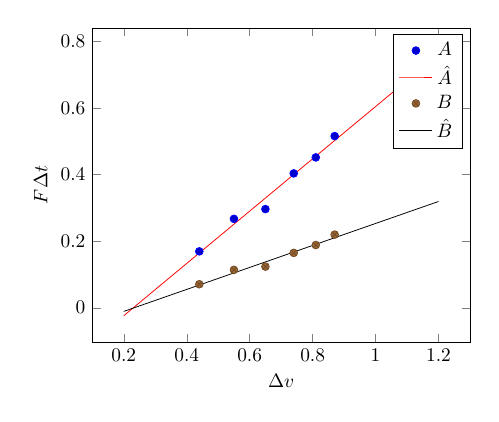
\begin{tikzpicture}[scale=0.7,transform shape]
        \begin{axis}[xlabel=$\Delta v$, ylabel=$F \Delta t$, domain=0.2:1.2]
            \addplot+[only marks] coordinates {
                (0.44, 0.1692)
                (0.55, 0.2668)
                (0.65, 0.2961)
                (0.74, 0.4032)
                (0.81, 0.4512)
                (0.87, 0.5152)
            };
            \addplot+[no markers] {0.785*x-0.181};
            \addplot+[only marks] coordinates {
                (0.44, 0.0706)
                (0.55, 0.1137)
                (0.65, 0.1235)
                (0.74, 0.1646)
                (0.81, 0.1882)
                (0.87, 0.2195)
            };
            \addplot+[no markers] {0.330*x-0.077};
            \legend{$A$, $\hat{A}$, $B$, $\hat{B}$}
        \end{axis}
    \end{tikzpicture}
    \caption{Plot of $v_f$ and $F \Delta t$.}
    \label{fig:graph}
\end{figure}

The graph can be seen in Figure \ref{fig:graph}. The line $\hat{A}$ is the best
fit line of the set of points $A$. The slope of $\hat{A}$ is around 0.785 kg.
0.785 kg should still include the 20 g of the mass, so 0.765 kg should be the
actual, real mass of the cart. \\

\noindent Okay. 0.765 kg is sizably greater than and off from 0.281 kg. Just
sayin'.

Let's do a little cheating. Obviously 0.47 N is way off of the expected value of
0.196 N, so let's replace $F$ with a constant value. This value? Well... oh, I
don't know, 0.196 N. Sounds like a nice number. Also considerably less than 0.47
N, but I'm not one to talk about size.

The graph of the corrected $F$ can be seen in Figure \ref{fig:graph}. As before,
the line $\hat{B}$ is the line of best fit for the set of points $B$. The slope
of $\hat{B}$, however, is about 0.330 kg. 0.330 kg minus the mass equates to
0.310 kg, which \emph{really} should be the actual, real mass of the cart.

\section{Conclusion} \label{sec:conclusion}

When the faulty $F$ data is used to calculate $m$, we get a percent error of
about 172.2\% bigger $m$ than expected. That's... pretty bad. However, with my
revolutionary technique of falsifying the $F$ data, we get a percent error of
about 10.3\%. That's pretty good!

However, why was $F$ faulty? Since "my teammates messed up" is not a valid
line of reasoning, it may be more accurate to say that "the sensor cart messed
up." In other words, I believe it could have been the sensor cart measuring $F$
incorrectly, and giving us garbage data. That would not explain how $F$ managed
to stay consistent between multiple trials, however.

If we assumed that "my teammates messed up" could be valid, it could also be
that $F$ was not measured in newtons, but instead in some other, evil
measurement. Such as $\text{lb} \cdot \text{ft/s}^2$, if the recording software
allows.

What if \emph{I} messed up? Not in a philosophical way, but instead in a lesser,
more benign way.  It seems unlikely as well, but I could have accidentally
picked the wrong mass when I set up the half-Atwood machine. That would explain
the increased $F$, but it would also contradict the fact that when the $F$ data
is ignored, we get a pretty good percent error.

If $F$ is incorrect, is any of the other data even correct? What about $v_f$? If
we assume that $x$ from \ref{fig:data} is correct (which I really hope is true),
we can actually guess the $v_f$. Since the mass hits the ground when the cart is
30 cm away from the pulley, we can solve for $v_f$ using $KE = \Delta U_g$.
Using $x = 50$ cm:

\begin{align*}
    \frac{1}{2} \cdot 0.301 \text{ kg} \cdot v_f^2 &= 0.020 \text{ kg} \cdot 9.8 \text{ m/s}^2 \cdot 0.20 \text{ m} \\
    v_f &= 0.51 \text{ m/s}
\end{align*}

Eh, 0.51 m/s is pretty close to 0.44 m/s. That's around a 13.7\% error, which
itself is closer to the 10.3\% error for the fake-$F$ data.

\end{document}

